

%%%%%%%%%%%%%%%%%%%%%%%%%%%%%%%%%%%%%%%%%%%%%%%%%%%%%%
\section{Design / Proposed Approach}
\label{sec:design}

\subsection{Overview and Goals}
In our initial simple system, "Iroko", a centralized controller regulates all 
node traffic by rate-limiting end-hosts. We have opted for a centralized 
manager in favor of a distributed protocol to leverage the advantages of a 
global network view.~\footnote{For now, we do not expect our design to scale up 
to thousands of switches. Iroko is intended for small to mid-tier size data 
centers, which may benefit from a simplistic, centralized scheduling model.}
By polling each switch individually for port and utilization statistics we are 
able to infer a global traffic matrix, which we can amalgamate with static 
routing and topology information. 

Iroko guarantees minimal congestion and low average access latency. Reducing 
network-global packet loss and jitter is the priority and objective function of 
the arbiter, which will enforce these goals by restricting host bandwidth. In 
an ideal Iroko system, packet-loss will only rarely, if ever, occur. In respect 
to the free lunch theorem we aim to trade off maximum bandwidth utilization for 
optimal system stability and reliable latency.

It is important to note that routing decisions are not in the current scope of 
Iroko. While it may certainly beneficial to include dynamic and adaptive 
routing decisions in a predictive scheduler, we do not include these features 
in the current system due to time and complexity limitations. Iroko operates on 
static flow routes defined and generated by ECMP. It is assumed that these 
routes will not vary substantially and that the computed ECMP forwarding hash 
is consistent.


\subsection{Controlling traffic flow}
Rate-limiting is performed on the granularity of the IP protocol, allowing us 
to restrict traffic to specific hot regions and to package flows into groups.
End-hosts are guaranteed a limited amount of bandwidth which they may send to 
each destination address. The traffic window size for any flow is calculated 
based on the host's current traffic availability. Total bandwidth of a group of 
flows may never exceed the imposed bandwidth limitation, but nodes are free to 
distribute the allocated resources on singular subflows.

The central arbiter enforces these bandwidth and access limitations by 
assigning "tokens" to nodes. These tokens are plain information packets 
specifying the affected destination address flow, its bandwidth guarantee, and 
the expiration time. Tokens act as the rate-limiter of the system and form a 
queue each end-host will cycle through.

When a node opens a flow, it will look up the current bandwidth restriction for 
the destination IP in its token database and calculate the maximum congestion 
window possible for the particular TCP connection. In our simple design, flows 
are always assigned a fair fraction.

Once a token has expired for a particular flow-group, the restrictions of the 
next token in the queue will be applied. This mechanism is the underlying basis 
for a predictive access control algorithm and does not require any application 
level modification. On end-hosts, only the transport layer services will have 
to be modified.

\subsection{Adapting traffic flow}

Initially, the controller will compute optimal route configuration based on the 
topology and link bandwidth using a simple heuristic bin-packing approach. 
End-hosts will be initialized with a fixed low-to-medium bandwidth guarantee 
that will be adjusted over time. This bandwidth guarantee will be below the 
host's proportional bi-section bandwidth that would be used to reach any other 
host. That is, if every end host transfers using the full bandwidth initially 
allocated to it,  there would be no dropped packets due to congestion.

Of course, this would vastly underutilize network resources, thus the 
controller will dynamically adjust these allocations to ensure that hosts that 
require the bandwidth are allocated it, while host that are not currently 
utilizing all their allocated bandwidth have their allocated bandwidth reduced. 
To avoid starving hosts, some small amount of bandwidth must always be 
allocated to a given host even if it not utilizing network resources. Thus, the 
network, by design, will never reach 100\% utilization.

Conversely however one should rarely see dropped packets due to network 
congestion. Furthermore, the controller must be able to react quickly to 
changing bandwidth needs for hosts. Ideally, using a predictive method.

\begin{figure}
\centering
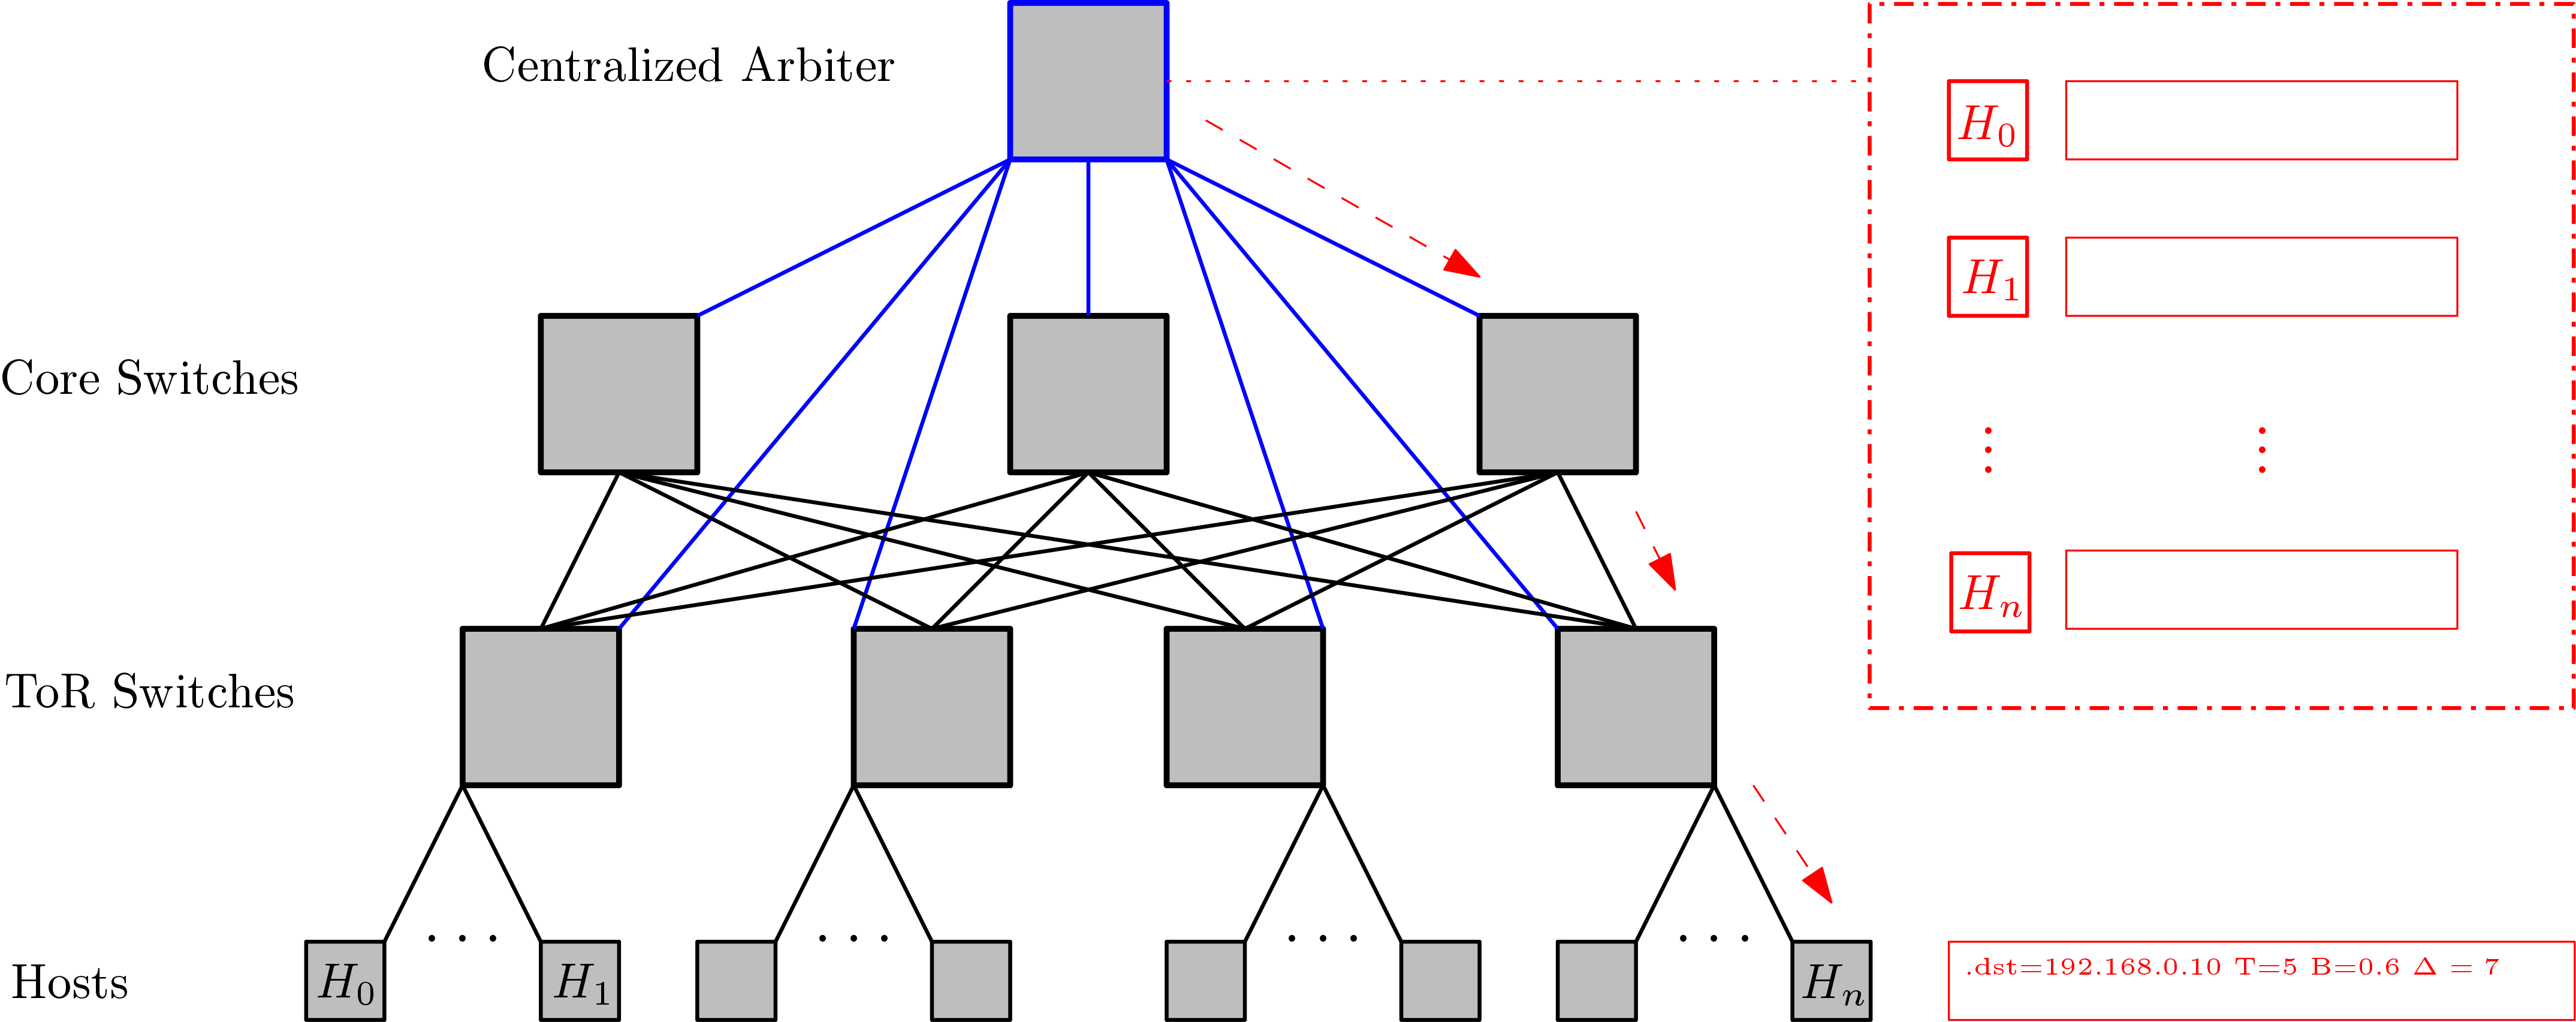
\includegraphics[width=1\linewidth]{Topology3}
\caption{Simple sketch of the Iroko architecture. A central scheduler maintains 
a consistent view of the current network activity and computes the optimal 
end-host bandwidth distribution. Bandwidth is enforced at end-hosts on a per-IP 
basis.}
\label{fig:Topology3}
\end{figure}

\subsection{Statistical System}
One potential implementation for our arbiter is to use reinforcement learning. 
In reinforcement learning, an agent (in our case the arbiter) performs actions 
in the environment and receives a reward signal from the environment to adjust 
its decisions in the next epoch ~\cite{Sutton:1998:IRL:551283}. The reward is 
generally used to represent the goal the agent is trying to achieve. The agent 
can freely choose whatever actions are necessary to achieve this goal 
~\cite{Sutton:1998:IRL:551283}.

The environment in this case is defined as the statistics collected from each 
switch. This decision is based on the fact that this data is easy to collect 
and provides a current snapshot of the performance of the network. We wish to 
optimize over the packet loss, and define the reward to be good if packet loss 
is decreasing (+1 reward); bad if it is increasing ( -1 reward); and acceptable 
if packet loss remains the same within a threshold (0 reward). Using this 
representation, we take full advantage of all the information provided in our 
data center; This representation is replicable and can be applied beyond the 
scope of this project.
 
Given the data center assumption, the number of end-hosts is known in the 
topology. We can define our arbiter's actions as a discretized representation 
among an n-dimensional vector where each cell is one of three values: increase 
decrease, or maintain the allocated bandwidth. This representation offers 
sufficient complexity. There are $3^n$ possible actions to perform and to 
achieve optimal results the agent must explore the environment extensively, 
precluding a significantly larger action space.

A potential improvement to our representation is a hierarchical learning agent. 
In this case, our arbiter would manage agents for each host and these 
sub-agents would manage their respective host whether to increase, decrease, or 
maintain bandwidth for their particular host. This problem can be referred to 
as hierarchical reinforcement learning~\cite{Borga1993}, but may prove to be 
beyond the scope of our current proposed solution, although has the added 
benefit of solving a set of sub-problems to address the global problem of 
packet loss and simplifies the representation spaces in the sub-problems.

Thus we frame our problem as one which can now be solved using techniques in 
reinforcement learning. A classic algorithm to consider is the use of 
SARSA~\cite{Sutton:1998:IRL:551283}, which is an online temporal difference 
algorithm used in classical reinforcement learning problems. One advantage of 
SARSA is its online nature~\cite{Sutton:1998:IRL:551283} which promotes more 
conservative decisions. Given full representation of our environment and 
actions, we can store information in an artificial neural network which is 
another popular choice in reinforcement learning literature. This model would 
store the reward signal information that is used to make future action choices, 
and is a theoretically proven function approximator which has made intractable 
environmental representations manageable~\cite{Sutton:1998:IRL:551283}.


%Using this model, we hope to achieve near 0% packet loss and provide a 
%%solution that gets somebody fired at google for not having tried it first.

